\documentclass[fleqn,11pt]{article}
\usepackage[utf8]{inputenc}

\usepackage{amsmath}
\usepackage{amssymb}
\usepackage{caption}
\usepackage{fullpage}
\usepackage{graphicx}
\usepackage{hyperref}
\usepackage{mathtools}
\usepackage{titling}

\setlength\parindent{0pt}
\setlength\mathindent{0pt}

\newcommand{\subtitle}[1]{%
  \posttitle{%
    \par\end{center}
    \begin{center}\large#1\end{center}
    \vskip0.5em}%
}

\title{Analýza clusterů pomocí $\chi^2$ testu}
\subtitle{Zápočtová práce z A0B01PSI, ČVUT FEL}

\author{Jonáš Amrich}
\date{2013}

\begin{document}
    \maketitle
    \section{Úvod}
    Pro svou zápočtovou práci jsem si vybral problém, se kterým jsem se setkal v jiném projektu na ČVUT. Cílem je identifikace clusterů v daném vektorovém prostoru. Jednou z možností, která není příliš výpočetně náročná a kterou můžeme vyvrátit existenci clusterů v prostoru, je analýza vzájemných vzdáleností (pairwise distances) jednotlivých bodů. V případě, že prostor obsahuje clustery, rozdělení vzájemných vzdáleností by mělo být směsí dvou rozdělení - \textit{inter}clusterových a \textit{intra}clusterových vzdáleností. V opačném případě, kdy body v prostoru netvoří clustery, předpokládáme, že je rozdělení vzájemných vzdáleností normální.

    \section{Data}
    Mým datasetem jsou vzájemné vzdálenosti vektorů, které byly vytvořeny pomocí nástroje word2vec \cite{mikolov2013efficient}. Dataset "99k" obsahuje cca 99 tisíc vektorů slov v 600 dimenzích, které byly natrénovány pomocí anglické wikipedie \cite{wiki}.
    Pro účely testu diskretizuji rozdělení vzdáleností do 50, respektive 100 disjunktních tříd. Vzhledem k množství dat jsem z těchto tříd pro test použil jen ty, jejichž teoretická četnost přesahovala $10^8$ (v grafu znázorněno žlutým pruhem).

    \section{Test}

    $X$ - rozdělení vzájemných vzdáleností\\
    $\mu_X \doteq 5.947$\\
    $\sigma_X \doteq 1.091$\\
    \\
    $N$ - normální rozdělení\\
    $N = N(\mu_X, \sigma_X^2)$\\
    \\
    $H_0$: Vzájemné vzdálenosti mají normální rozdělení na hladině významnosti 5\%\\

    % 50 tříd
    \begin{table}[htp]
        \footnotesize
        \caption*{$\chi^2$ test, 50 tříd}
        \centering
        \begin{tabular}{|l|l|l|l|l|l||l|}
        \hline
         & 8 & 9 & ... & 19 & 20 & \\ \hline
        N& 0.023 & 0.038 & ... & 0.037 & 0.022 & 1 \\ \hline
        X& 64\,074\,592 & 192\,428\,527 & ... & 85\,435\,352 & 54\,499\,482 & 4\,894\,512\,330 \\ \hline
        teoretická četnost& 112\,932\,410 & 188\,413\,183 & ... & 182\,259\,731 & 108\,521\,033 & 4\,894\,512\,330 \\ \hline
        příspěvek k $\chi^2$& 21\,137\,301 & 85\,572 & ... & 51\,437\,365 & 26\,891\,819 & 592\,417\,157 \\ \hline
        \end{tabular}
    \end{table}

    % 100 tříd
    \begin{table}[htp]
        \footnotesize
        \caption*{$\chi^2$ test, 100 tříd}
        \centering
        \begin{tabular}{|l|l|l|l|l|l||l|}
        \hline
         & 19 & 20 & ... & 36 & 37 & \\ \hline
        N& 0.024 & 0.029 & ... & 0.028 & 0.023 & 1 \\ \hline
        X& 117\,469\,475 & 168\,066\,472 & ... & 78\,797\,567 & 61\,423\,024 & 4\,894\,512\,330 \\ \hline
        teoretická četnost& 117\,482\,714 & 143\,118\,546 & ... & 139\,366\,843 & 114\,023\,788 & 4\,894\,512\,330 \\ \hline
        příspěvek k $\chi^2$& 1 & 4\,348\,835 & ... & 26\,323\,601 & 24\,265\,466 & 371\,332\,014 \\ \hline
        \end{tabular}
    \end{table}


    %\[
    %    T \coloneqq \sum_{i=1}^k \frac{(n_i - np_i)^2}{np_i}
    %\]
    $T_{50} = 592\,417\,157\\$
    $T_{100} = 371\,332\,014\\$

    $q_{\chi^2(50)}(95) =  67.50$\\
    $q_{\chi^2(50)}(99.95) =  89.56$\\
    \\
    $q_{\chi^2(100)}(95) =  124.34$\\
    $q_{\chi^2(100)}(99.95) =  153.16$\\
    \\
    $T_{50} > q_{\chi^2(50)}(99.95) > q_{\chi^2(50)}(95)$\\
    $T_{100} > q_{\chi^2(100)}(99.95) > q_{\chi^2(100)}(95)$\\
    \\
    Už při pohledu na graf je vidět, že testovací statistika bude řádově převyšovat jak 95\%, tak 99.95\% kvantil $\chi^2$ rozdělení, hypotézu tedy zamítáme.

    \begin{figure}[htp]
        \footnotesize
        \centering
        \caption*{Histogram vzájemných vzdáleností, 50 tříd}
        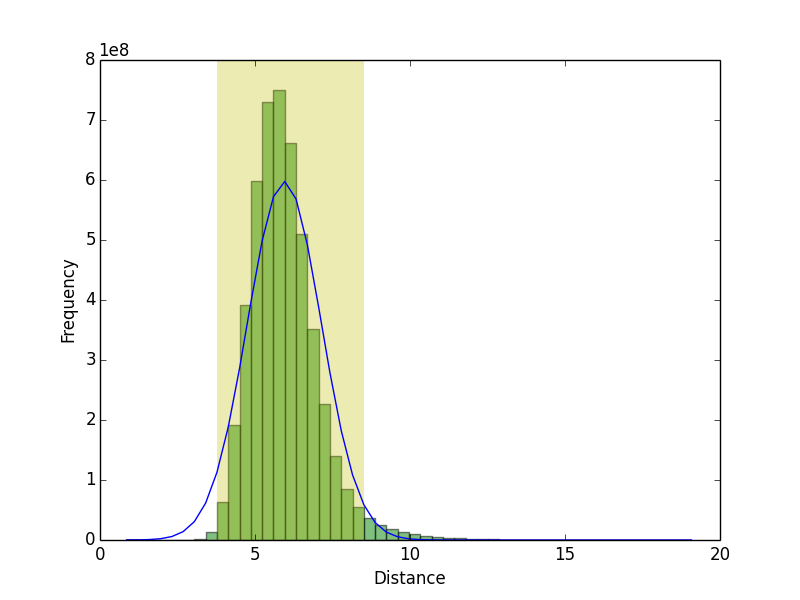
\includegraphics[width=13cm]{figures/enwiki-99k-50bins.png}
    \end{figure}

    \begin{figure}[htp]
        \footnotesize
        \centering
        \caption*{Histogram vzájemných vzdáleností, 100 tříd}
        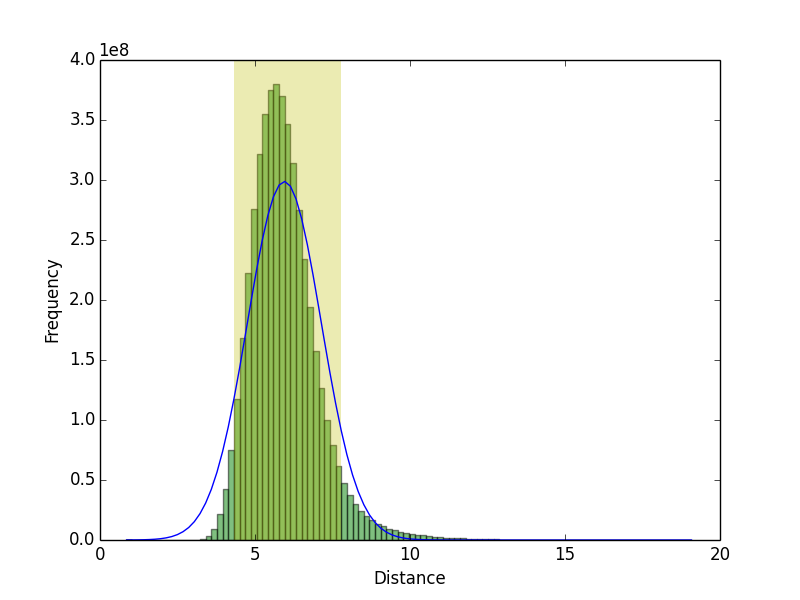
\includegraphics[width=13cm]{figures/enwiki-99k-100bins.png}
    \end{figure}

    \renewcommand\refname{\section{Reference}}
    \bibliographystyle{unsrt}
    \bibliography{bibtex/mikolov2013efficient,bibtex/ghrepo,bibtex/wiki}
\end{document}